\chapter{Introducci\'on}
\label{intro}
%\newquote{Who Watches the Watchmen?}{Watchmen - Alan Moore}

En los últimos 10 años, la revolución que ha causado el empleo de teléfonos inteligentes en la población 
ha permitido masificar el uso del internet y podríamos decir sin temor a equivocarnos, la democratización de su uso.
 La consecuencia es que las personas están más comunicadas y/o conectadas en tiempo real a través  de comunidades 
 en internet, las cuales son más conocidas con el nombre de “redes sociales”, el caso más emblemático de su empleo 
 en una revolución políticas sucedió entre los años 2011 y 2012 , con el movimiento denominado  “Primavera Árabe” (1), 
 donde las redes sociales tuvieron una vital importancia para la organización de este movimiento, siendo las redes 
 sociales más empleadas Facebook y Twitter. 
      
Twitter como se mencionó anteriormente es una red social donde un usuario, que previamente se ha registrado, 
puede enviar mensaje de texto sobre un tema que él considere importante o puede interactuar con otros mensajes 
dando a conocer su punto de vista; el texto enviado es conocido como tweets y tiene un máximo de 280 caracteres. 
En la página de Twitter, la empresa se define a sí misma con las siguientes palabras “lo que está pasando en el 
mundo y los temas sobre los que está hablando la gente.” (2). Un componente opcional en los tweets es que incluye 
su geolocalización, lo cual es una pieza importante en el análisis del comportamiento porque nos permite determinar 
la opinión de las personas por zonas geográficas. 

La situaci\'on en el Per\'u no es ajena, de acuerdo al estudio de mercado realizado por la consultora CPI (Compa\~nia Peruana de Estudios de Mercados y Opini\'on P\'ublica S.A.C.) sobre el uso de redes sociales en Lima de agosto del 2018 , se evidencia el uso de Facebook como la red social mas popular con el 72.7\%, seguido de WhatsApp al 68.5\%, Instragram al 25.0\% y como cuarto puesto a Twitter con el 12.7\%. 


\begin{figure}
\centering
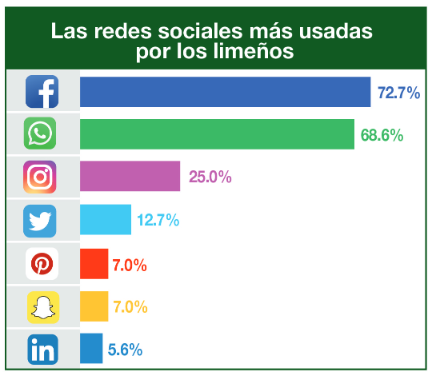
\includegraphics[scale=0.7]{chapters/img/Ch01_UsoRedesSocialesLima.PNG}
\caption{Redes Sociales mas usada por los lime\~nos - Agosto 2018 - Fuente : CPI}
\end{figure}
%\\
%El uso generaci\'on de la red social es mostrado a continuaci\'on 

\begin{figure}
\centering
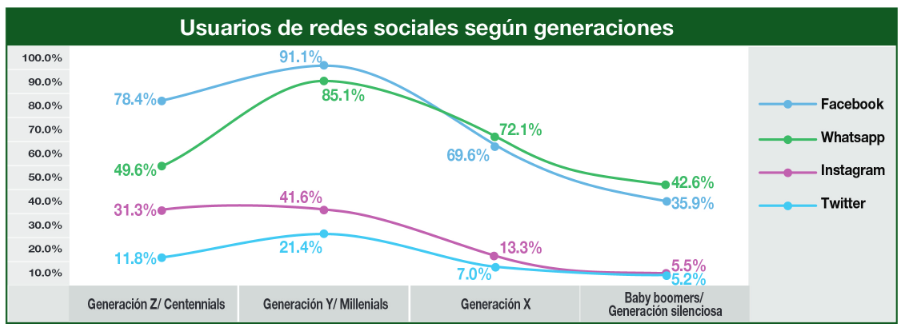
\includegraphics[scale=0.5]{chapters/img/Ch01_UsoRedesSocialesGeneracion.PNG}
\caption{Uso de redes sociales seg\'un generaci\'on - Agosto 2018 - Fuente : CPI}
\end{figure}

% En el presente documento se realizará un estudio de investigación sobre las  opiniones que tienen el consumidor ime\~no sobre las tiendas por departamento; se usará como datos la información de la red social Twitter, obteniéndola de 5 geolocalizaciones correspondiente a  las denominadas 5 Limas: Lima Sur, Lima Norte, Lima Este y Lima Centro. Para tal fin se empleará el análisis de sentimiento para determinar las preferencias de los limeños, los tweets serán obtenidos en geolocalizaciones de las 5 Limas: Lima Sur, Lima Norte, Lima Este, Lima Centro y Lima Moderna; y para analizar los datos se usará la técnica de text mining, el cual es el proceso de obtener conocimiento implícito desde una información basado en texto. \\

%La finalidad de esta tesis es poder definir una metodolog\'ia para el an\'alisis en la red social Twitter sobres las opiniones de los usuarios  de mercado basada en text mining que nos permite reducir en tiempo y costo con un estudio de mercado tradicional en el campo de marketing. 

\cleardoublepage